\section{Implementation Details}

Note that the reformulation mentioned above does not neccesiate any
change in the proposed optimization algorithm as we still need to
follow the block-gradient descent method (since even the reformulation
does not make the objective jointly convex in $X,W$ and $X$ is still
required to be discreet). In our implementation, we experiment with both the relaxed formulation as well as the original formulation (with mometum penalty modified to be convex). In this section, we descibe the finer implementation details of our algorithm.


\subsection{Initialization}

We have shown earlier that the objective function is not jointly convex
over $X,W$. So, the solution that the algorithm converges to is highly
dependent on the initialization. Therefore, we need to determine a
reasonable initialization for the weight variables. We experiment
with two standard optical flow algorithms \cite{HornSchunk}, \cite{LukasKanade} to
initialize the flow variables for each video frame (and thus the weight
variables). The implementation is as follows -

\begin{algorithm}[H]
\framebox{\begin{minipage}[t]{1\columnwidth}%
function $generatePriors(I)$
\begin{itemize}
\item for $t=1:T-1$

\begin{itemize}
\item $(U_{t},V_{t})=opticalFlow(I_{t},I_{t+1})$
\end{itemize}
\item $W\leftarrow UVtoWeights(U,V)$
\item return $W$\end{itemize}
%
\end{minipage}}\caption{$generatePriors(I)$}
\end{algorithm}



\subsection{Unary Appearance Cost}

To determine the unary costs, we learn a foreground model based on
the intitial frame segmentation. We train a random forest classifier
using for patches using the patches around foreground pixels in the
intial frame as positive examples and the patches around other pixels
as negative examples. We then predict the probability of a pixel in
a given frame being a foreground pixel by classifying the patch surrounding
it using the trained classifier. The foreground label cost for the
given pixel is stored as $1-classifierProbability(I_{ijt})$.

\begin{figure}[H]
\begin{centering}
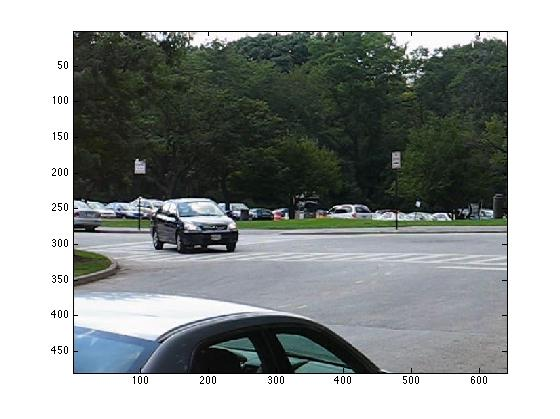
\includegraphics[scale=0.2]{figures/UnaryCostGT}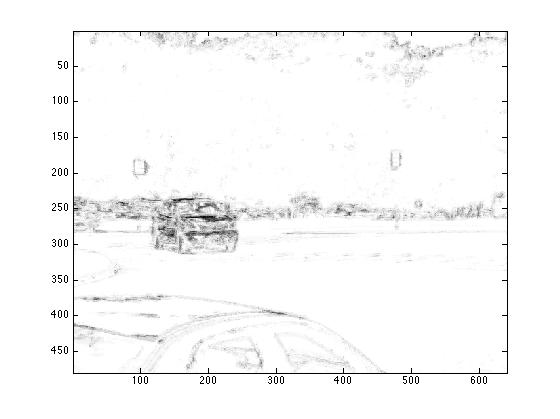
\includegraphics[scale=0.2]{figures/UnaryCost}\caption{Appearance Costs visualization : Low intensity represents low foreground cost
(object being tracked is upper car)}

\par\end{centering}

\end{figure}



\subsection{Finding flows given label assignments}


\subsection{Propogating labels}